% =====================================================================
%  PLANTILLA DE TESIS — CISE, Universidad Autónoma de Coahuila
%  Archivo principal: es el ÚNICO que se compila.
%
%  Estructura:
%    main.tex                 <- este archivo (orden de las secciones)
%    referencias.bib          <- bibliografía (exportada de Zotero)
%    codigo/configuracion.tex <- paquetes, márgenes, interlineado, estilos
%    codigo/portada.tex       <- portada y datos de la tesis
%    codigo/introduccion.tex
%    codigo/capitulo_1.tex ... codigo/capitulo_4.tex
%    codigo/conclusiones.tex  <- conclusiones y recomendaciones
%    codigo/anexos.tex
%    figuras/                 <- logos e imágenes (PDF, PNG o JPG)
%
%  Compilar con pdfLaTeX + Biber (Overleaf lo hace automáticamente).
% =====================================================================
\documentclass[12pt, oneside, letterpaper]{book}

% La configuración va en el preámbulo, donde \include no está permitido;
% por eso se carga con \input.
% =====================================================================
%  CONFIGURACIÓN — paquetes, página, interlineado y estilos
%  Formato basado en la plantilla de tesis del CISE.
%  Un cambio aquí afecta a toda la tesis.
% =====================================================================

% ----------------------------- IDIOMA --------------------------------
\usepackage[utf8]{inputenc}
\usepackage[T1]{fontenc}
\usepackage[american, spanish, es-noquoting, es-nodecimaldot, es-tabla,
            es-lcroman]{babel}
% es-tabla: "Tabla" en lugar de "Cuadro"; es-nodecimaldot: 0.5 y no 0'5
% es-lcroman: páginas romanas en minúscula normal (ii, iii); sin esta
%             opción, babel las escribe en versalitas
\usepackage{csquotes}

% Los anexos se titulan "Anexo A" en lugar de "Apéndice A"
\addto\captionsspanish{\renewcommand{\appendixname}{Anexo}}

% ----------------------------- FUENTE --------------------------------
% Palatino (TeX Gyre Pagella) en el texto y en todas las ecuaciones,
% incluidos los símbolos (=, +, \sum, \int, \mathcal...). newpxmath carga
% amsmath y los símbolos de amssymb, así que no cargue amssymb aparte.
% amsmath y amsthm deben cargarse ANTES que newpxmath.
\usepackage{amsmath, amsthm}
\usepackage{newpxtext}
\usepackage{newpxmath}
\usepackage{microtype}

% ------------------------ GEOMETRÍA DE PÁGINA ------------------------
\usepackage[paper=letterpaper, centering, includehead]{geometry}
\geometry{tmargin=2cm, bmargin=2.5cm, lmargin=2cm, rmargin=2cm}
\geometry{head=0cm, foot=0cm, headsep=0cm, footskip=0.75cm}
\geometry{columnsep=0.5cm}

% ---------------------- PÁRRAFOS E INTERLINEADO ----------------------
\setlength{\parskip}{0.3cm}         % Espacio entre párrafos
\setlength{\parindent}{0cm}         % Sin sangría
\usepackage{setspace}
\setstretch{1.3}                    % Interlineado (1.5 = \onehalfspacing)

% ------------------------ ESTILO DE CAPÍTULOS ------------------------
\usepackage[Glenn]{fncychap}
\ChNameVar{\bfseries\Large\rmfamily}
\ChNumVar{\Huge}
\ChTitleVar{\bfseries\large\rmfamily}
\ChRuleWidth{1pt}

% ---------------------- ENCABEZADOS Y PIES ---------------------------
\usepackage{fancyhdr}
\pagestyle{fancy}
\fancyhf{}                          % Limpia encabezado y pie
\fancyfoot[R]{\thepage}             % Número de página abajo a la derecha
\renewcommand{\headrulewidth}{0pt}
\renewcommand{\footrulewidth}{0.5pt}
% Primera página de cada capítulo: mismo pie
\fancypagestyle{plain}{%
  \fancyhf{}\fancyfoot[R]{\thepage}%
  \renewcommand{\headrulewidth}{0pt}\renewcommand{\footrulewidth}{0.5pt}}

% --------------------------- MATEMÁTICAS -----------------------------
\newtheorem{teorema}{Teorema}[chapter]
\newtheorem{corolario}[teorema]{Corolario}
\newtheorem{lema}[teorema]{Lema}
\newtheorem{proposicion}[teorema]{Proposición}
\theoremstyle{definition}
\newtheorem{definicion}{Definición}[chapter]
\newtheorem{ejemplo}{Ejemplo}[chapter]

% ------------------------ TABLAS Y FIGURAS ---------------------------
\usepackage{graphicx}
\graphicspath{{figuras/}}           % Las imágenes se buscan en figuras/
\usepackage{booktabs}
\usepackage{multirow}
\usepackage{longtable}
\usepackage{threeparttable}
\usepackage{caption}
\captionsetup{font=small, labelfont=bf}
\captionsetup[table]{skip=10pt}
\usepackage{subcaption}
\usepackage{float}
\usepackage[dvipsnames]{xcolor}

% ------------------------------ LISTAS -------------------------------
\usepackage{enumitem}
\setlist{itemsep=0.1cm, topsep=0.1cm}

% --------------------------- OTROS -----------------------------------
\usepackage{multicol}
\usepackage[nohyperlinks]{acronym}  % Siglas: \ac{INEGI} (ver codigo/siglas.tex)
\usepackage{lipsum}                 % Texto de relleno: borrar al terminar
\SetLipsumLanguage{spanish}         % Evita el aviso por el idioma "latin"

% --------------------------- MARCA DE AGUA ---------------------------
% Para versiones de revisión, descomente las siguientes líneas.
%\usepackage{draftwatermark}
%\SetWatermarkText{BORRADOR}
%\SetWatermarkLightness{0.93}
%\SetWatermarkScale{0.75}

% -------------------------- BIBLIOGRAFÍA -----------------------------
% APA 7 (paquete biblatex-apa). No agregue opciones como maxcitenames:
% style=apa ya aplica las reglas de APA (et al., número de autores, etc.).
% Para un autor-año genérico en lugar de APA, cambie la línea por:
%   \usepackage[backend=biber, style=authoryear, maxcitenames=2,
%               maxbibnames=10, uniquename=false, dashed=false]{biblatex}
\usepackage[backend=biber, style=apa]{biblatex}
\addbibresource{referencias.bib}

% ------------------------- COMANDOS PROPIOS --------------------------
\newcommand{\E}{\mathbb{E}}         % Esperanza
\newcommand{\R}{\mathbb{R}}         % Números reales
\newcommand{\ingles}[1]{\foreignlanguage{american}{\emph{#1}}} % Términos en inglés

% ---------------- ENLACES Y REFERENCIAS CRUZADAS ---------------------
% Siempre al final del preámbulo y en este orden.
\usepackage[hidelinks, bookmarksnumbered]{hyperref}
\usepackage[spanish]{cleveref}
\crefname{chapter}{capítulo}{capítulos}
\crefname{section}{sección}{secciones}
\crefname{equation}{ecuación}{ecuaciones}
\crefname{table}{tabla}{tablas}
\crefname{figure}{figura}{figuras}
\crefname{appendix}{anexo}{anexos}


% ---------------------- COMPILAR SOLO ALGUNAS SECCIONES --------------
% Para compilar más rápido mientras escribe, descomente y deje solo las
% secciones en las que está trabajando. La numeración del resto se conserva.
%\includeonly{
%codigo/introduccion,
%codigo/capitulo_1,
%}

\begin{document}

% ------------------------------ PORTADA ------------------------------
% Numeración interna "A" (no se imprime) para que la portada no comparta
% el número 1 con el primer capítulo y los enlaces del PDF no se confundan.
\pagenumbering{Alph}
% =====================================================================
%  PORTADA — edite solo los datos entre llaves
%
%  Los espacios verticales están ajustados para que el título, el nombre
%  y el comité queden a la misma altura que en la portada anterior del
%  CISE (al empastar, la tapa tiene un recuadro que debe coincidir).
%  No cambie los \vspace ni los tamaños de letra.
% =====================================================================
\newcommand{\titulotesis}{Título de la tesis}
\newcommand{\autortesis}{Nombre Completo del Estudiante}
\newcommand{\programa}{Doctorado en Economía Regional}
\newcommand{\grado}{Doctor(a) en Ciencias en Economía Regional}
\newcommand{\director}{Dr(a). Nombre del Director(a) (CISE)}
\newcommand{\codirector}{Dr(a). Nombre del Codirector(a) (CISE)}
\newcommand{\lectoruno}{Dr(a). Nombre del Lector(a)}
\newcommand{\lectordos}{Dr(a). Nombre del Lector(a)}
\newcommand{\lugar}{Saltillo, Coahuila}
\newcommand{\fecha}{Mes de 2026}

% Se usan en el Resumen, el Abstract y los metadatos del PDF
\newcommand{\palabrasclave}{palabra uno, palabra dos, palabra tres}
\newcommand{\keywordsingles}{keyword one, keyword two, keyword three}
\newcommand{\codigosjel}{R11, R12, O18}   % https://www.aeaweb.org/jel/guide/jel.php

% Metadatos del PDF (los leen los repositorios institucionales y buscadores)
\hypersetup{
  pdftitle    = {\titulotesis},
  pdfauthor   = {\autortesis},
  pdfsubject  = {Tesis de \programa, CISE, Universidad Autónoma de Coahuila},
  pdfkeywords = {\palabrasclave},
}

\thispagestyle{empty}
\begingroup
\centering
\singlespacing
\setlength{\parskip}{0pt}   % Sin espacio extra entre párrafos en la portada

% Logos (Manual de Marca UAdeC, 11/03/2026): la Marca Institucional va
% primero y con mayor peso que el logo del CISE; mínimo 3 cm de largo.
% Para imprimir en blanco y negro use uadec_marca_institucional_negro.
\begin{minipage}[c]{0.5\textwidth}
  \raggedright
  
\includegraphics[height=1.6cm]{uadec_marca_institucional}
\end{minipage}%
\hfill
\begin{minipage}[c]{0.5\textwidth}
  \raggedleft
  
\includegraphics[height=0.85cm]{cise}
\end{minipage}\par

\vspace{0.24cm}
{\large\bfseries CENTRO DE INVESTIGACIONES SOCIOECONÓMICAS\par}
\vspace{0.03cm}
{\large\bfseries \MakeUppercase{\programa}\par}

\vspace{0.74cm}
{\Large TESIS\par}

\vspace{1.54cm}
{\Large\bfseries \titulotesis\par}

\vspace{0.39cm}
{\large que presenta como requisito parcial para obtener\\
el grado de \grado\par}

\vspace{0.37cm}
{\Large\bfseries \autortesis\par}

\vspace{1.99cm}
{\Large\bfseries Comité Evaluador:\par}
\vspace{0.44cm}
{\large
\begin{tabular}{rl}
  Director(a):   & \director \\
  Codirector(a): & \codirector \\
  Lector(a):     & \lectoruno \\
  Lector(a):     & \lectordos \\
\end{tabular}\par}

\vspace{0.74cm}
{\large \lugar\\ \fecha\par}

\endgroup
\clearpage
      % Sin número de página, como la original

% --------------------------- PRELIMINARES ----------------------------
\frontmatter                  % Numeración romana desde i

% % =====================================================================
%  DEDICATORIA — opcional. Para quitarla, comente su \include en main.tex
% =====================================================================
\thispagestyle{plain}
\vspace*{0.3\textheight}
\begin{flushright}
  \itshape
  A mi familia\ldots
\end{flushright}
  % Opcional: dedicatoria / agradecimientos

\tableofcontents              % Índice general
\listoffigures                % Índice de figuras
\listoftables                 % Índice de tablas

% ------------------------- CUERPO DE LA TESIS ------------------------
\mainmatter                   % Numeración arábiga desde 1
% =====================================================================
%  INTRODUCCIÓN — capítulo sin número
% =====================================================================
\chapter*{Introducción}
\addcontentsline{toc}{chapter}{Introducción}  % Lo agrega al índice
\markboth{Introducción}{Introducción}
% Sin \label: un capítulo sin número no se puede citar con \cref
% (tomaría el número del capítulo anterior). Escriba "la introducción".

% Contenido sugerido: planteamiento del problema, justificación, pregunta
% de investigación, objetivos, hipótesis y organización del documento.
% En un capítulo sin número use \section* (secciones sin número).

\section*{Planteamiento del problema}

\lipsum[1]

\section*{Objetivos}

\textbf{Objetivo general.} \lipsum[2][1-3]

\textbf{Objetivos específicos:}
\begin{enumerate}
  \item \lipsum[3][1]
  \item \lipsum[3][2]
  \item \lipsum[3][3]
\end{enumerate}

\section*{Hipótesis}

\lipsum[4][1-4]

\section*{Estructura de la tesis}

% Con \cref los números se actualizan solos si cambia el orden.
La tesis se organiza en cuatro capítulos. El \cref{cap:capitulo1} \ldots; el
\cref{cap:capitulo2} \ldots; el \cref{cap:capitulo3} \ldots y el
\cref{cap:capitulo4} \ldots. Finalmente se presentan las conclusiones y
recomendaciones.

% =====================================================================
%  CAPÍTULO 1 — Ejemplo: marco teórico (citas, notas al pie, definiciones)
% =====================================================================
\chapter{Título del capítulo 1}\label{cap:capitulo1}

\section{Introducción del capítulo}

% Citas automáticas desde referencias.bib:
%   \textcite{clave}  -> Autor (año)      \parencite{clave} -> (Autor, año)
La economía regional estudia la dimensión territorial de los procesos
económicos \parencite{capello2015}. \textcite{krugman1991} muestra que los
rendimientos crecientes pueden generar patrones de concentración
núcleo-periferia.\footnote{Las notas al pie se numeran automáticamente.}
\lipsum[5]

\section{Revisión de la literatura}

\subsection{Primer enfoque}

\lipsum[6]

\begin{definicion}\label{def:ejemplo}
Texto de la definición. Los términos en otro idioma se marcan con
\ingles{spillovers}.
\end{definicion}

\subsection{Segundo enfoque}

Para el caso mexicano, \textcite{esquivel1999} documenta convergencia regional,
en línea con \textcite{barro1992}. \lipsum[7]

\section{Consideraciones finales del capítulo}

\lipsum[8]

% =====================================================================
%  CAPÍTULO 2 — Ejemplo: metodología (ecuaciones y referencias cruzadas)
% =====================================================================
\chapter{Título del capítulo 2}\label{cap:capitulo2}

\section{Introducción del capítulo}

\lipsum[9]

\section{Modelo teórico}

% Ecuación numerada: \begin{equation} ... \label{eq:...} \end{equation}
Siguiendo a \textcite{mankiw1992}, la función de producción es
\begin{equation}
  Y_t = K_t^{\alpha} H_t^{\beta} (A_t L_t)^{1-\alpha-\beta},
  \qquad \alpha + \beta < 1. \label{eq:produccion}
\end{equation}

% Varias ecuaciones alineadas en el signo "=": entorno align
El problema del hogar y su Lagrangiano son:
\begin{align}
  \max_{c,\,\ell} \; & u(c, \ell) \quad \text{s.a.} \quad c = w(1-\ell) + y, \label{eq:problema}\\
  \mathcal{L} &= u(c,\ell) + \lambda\,[w(1-\ell) + y - c]. \label{eq:lagrangiano}
\end{align}

\section{Estrategia empírica}

El modelo econométrico es
\begin{equation}
  y_i = \beta_0 + \beta_1 x_i + \mathbf{z}_i^{\top}\boldsymbol{\gamma}
        + \varepsilon_i, \qquad \E[\varepsilon_i \mid x_i, \mathbf{z}_i] = 0,
  \label{eq:modelo}
\end{equation}
que se estima por mínimos cuadrados ordinarios
\parencite{wooldridge2010, angrist2009}. La \cref{eq:modelo} se deriva de la
\cref{eq:produccion}; los resultados se presentan en el \cref{cap:capitulo3}.

\section{Datos}

\lipsum[10]

% =====================================================================
%  CAPÍTULO 3 — Ejemplo: resultados (tablas y figuras)
% =====================================================================
\chapter{Título del capítulo 3}\label{cap:capitulo3}

\section{Estadísticas descriptivas}

La \cref{tab:descriptivas} resume las variables principales.

% Tabla con booktabs: \toprule, \midrule, \bottomrule, sin líneas verticales.
% Si la tabla la genera Stata/R/Python, guárdela en codigo/ y use
%   \input{codigo/tabla_resultados}
\begin{table}[htbp]
  \centering
  \caption{Estadísticas descriptivas}
  \label{tab:descriptivas}
  \begin{threeparttable}
  \begin{tabular}{lrrrr}
    \toprule
    Variable & Media & Desv.\ est. & Mínimo & Máximo \\
    \midrule
    Variable 1 (\%)     & 37.92 & 14.42 & 8.40 & 65.90 \\
    Variable 2 (años)   &  9.70 &  1.13 & 7.40 & 12.70 \\
    Variable 3          &  0.77 &  0.14 & 0.53 &  0.98 \\
    \bottomrule
  \end{tabular}
  \begin{tablenotes}[flushleft]\footnotesize
    \item \textit{Fuente:} elaboración propia con datos de \ldots
  \end{tablenotes}
  \end{threeparttable}
\end{table}

\section{Resultados principales}

La \cref{fig:ejemplo} muestra \ldots

\begin{figure}[htbp]
  \centering
  % Las imágenes se buscan en figuras/ (ver \graphicspath en configuracion.tex)
  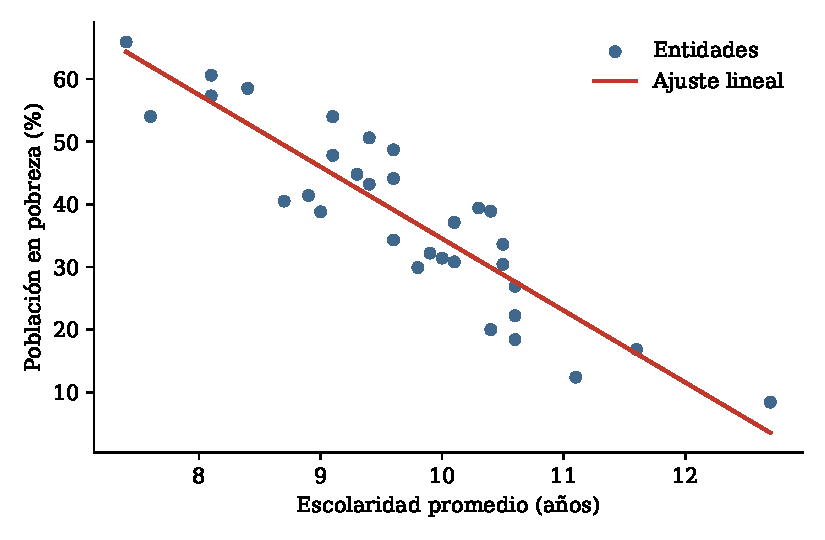
\includegraphics[width=0.75\textwidth]{figura_ejemplo}
  \caption{Título de la figura}
  \label{fig:ejemplo}
  \par\footnotesize\textit{Fuente:} elaboración propia.
\end{figure}

\lipsum[11-12]

% =====================================================================
%  CAPÍTULO 4 — Ejemplo: discusión (subfiguras y listas)
% =====================================================================
\chapter{Título del capítulo 4}\label{cap:capitulo4}

\section{Introducción del capítulo}

\lipsum[13]

\section{Análisis}

La \cref{fig:paneles} compara \ldots: el panel~\subref{fig:panel-a} \ldots
y el panel~\subref{fig:panel-b} \ldots

\begin{figure}[htbp]
  \centering
  \begin{subfigure}{0.48\textwidth}
    \centering
    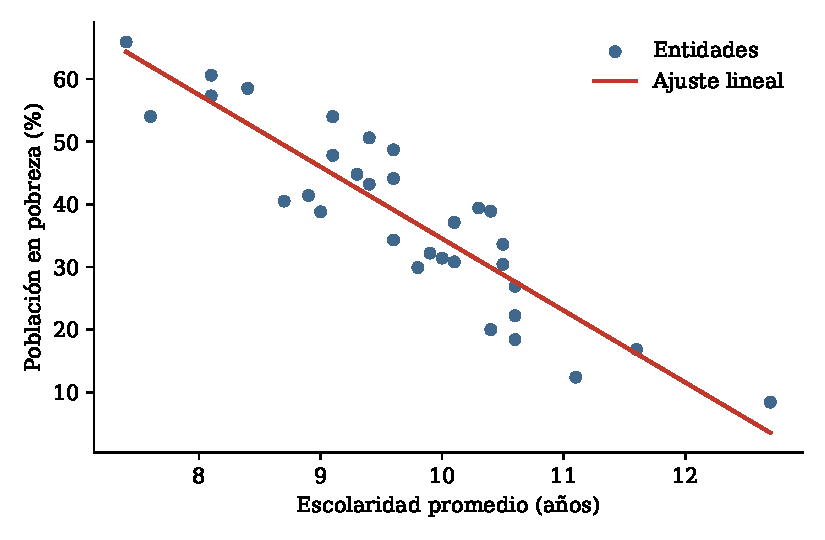
\includegraphics[width=\linewidth]{figura_ejemplo}
    \caption{Panel A}\label{fig:panel-a}
  \end{subfigure}\hfill
  \begin{subfigure}{0.48\textwidth}
    \centering
    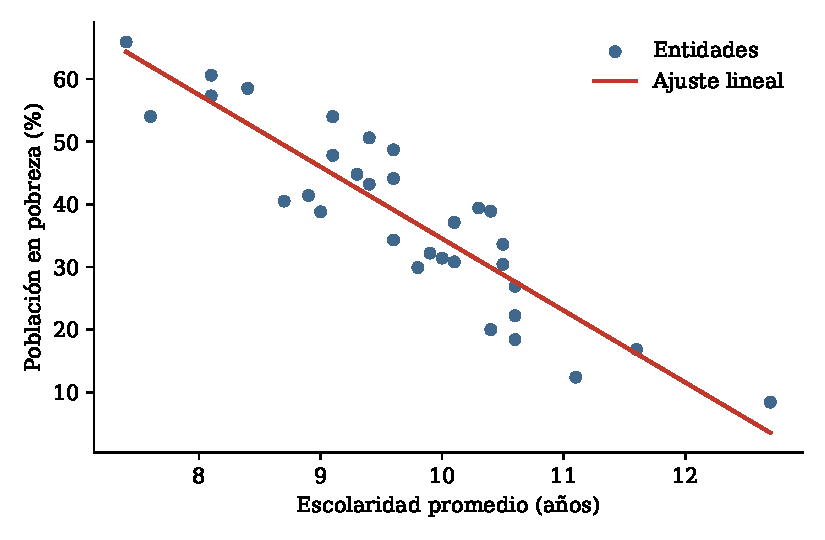
\includegraphics[width=\linewidth]{figura_ejemplo}
    \caption{Panel B}\label{fig:panel-b}
  \end{subfigure}
  \caption{Figura con dos paneles}
  \label{fig:paneles}
\end{figure}

\section{Discusión}

Los hallazgos principales son:
\begin{itemize}
  \item \lipsum[14][1-2]
  \item \lipsum[14][3-4]
  \item \lipsum[14][5-6]
\end{itemize}

\lipsum[15]

% =====================================================================
%  CONCLUSIONES Y RECOMENDACIONES — capítulo sin número
% =====================================================================
\chapter*{Conclusiones y recomendaciones}
\addcontentsline{toc}{chapter}{Conclusiones y recomendaciones}
\markboth{Conclusiones y recomendaciones}{Conclusiones y recomendaciones}
% Sin \label: un capítulo sin número no se puede citar con \cref
% (tomaría el número del capítulo anterior). Escriba "las conclusiones".

\section*{Conclusiones}
\addcontentsline{toc}{section}{Conclusiones}

\lipsum[16-17]

\section*{Recomendaciones de política}
\addcontentsline{toc}{section}{Recomendaciones de política}

\begin{enumerate}
  \item \lipsum[18][1-2]
  \item \lipsum[18][3-4]
\end{enumerate}

\section*{Limitaciones y agenda de investigación}
\addcontentsline{toc}{section}{Limitaciones y agenda de investigación}

\lipsum[19]


% ---------------------------- REFERENCIAS ----------------------------
\printbibliography[heading=bibintoc, title={Referencias}]

% ------------------------------- ANEXOS ------------------------------
% =====================================================================
%  ANEXOS — después de \appendix los capítulos se numeran A, B, C...
% =====================================================================
\appendix

\chapter{Definición de variables}\label{anx:variables}

\begin{table}[htbp]
  \centering
  \caption{Definición y fuente de las variables}
  \label{tab:variables}
  \begin{tabular}{lp{8cm}l}
    \toprule
    Variable & Definición & Fuente \\
    \midrule
    Variable 1 & Descripción de la variable 1 & INEGI \\
    Variable 2 & Descripción de la variable 2 & CONEVAL \\
    Variable 3 & Descripción de la variable 3 & Elaboración propia \\
    \bottomrule
  \end{tabular}
\end{table}

\chapter{Resultados complementarios}\label{anx:complementarios}

\lipsum[20]


\end{document}
